%% This is file `elsarticle-template-1-num.tex',
%%
%% Copyright 2009 Elsevier Ltd
%%
%% This file is part of the 'Elsarticle Bundle'.
%% ---------------------------------------------
%%
%% It may be distributed under the conditions of the LaTeX Project Public
%% License, either version 1.2 of this license or (at your option) any
%% later version.  The latest version of this license is in
%%    http://www.latex-project.org/lppl.txt
%% and version 1.2 or later is part of all distributions of LaTeX
%% version 1999/12/01 or later.
%%
%% Template article for Elsevier's document class `elsarticle'
%% with numbered style bibliographic references
%%
%% $Id: elsarticle-template-1-num.tex 149 2009-10-08 05:01:15Z rishi $
%% $URL: http://lenova.river-valley.com/svn/elsbst/trunk/elsarticle-template-1-num.tex $
%%
\documentclass[preprint,5p]{elsarticle}

%% Use the option review to obtain double line spacing
%% \documentclass[preprint,review,12pt]{elsarticle}

%% Use the options 1p,twocolumn; 3p; 3p,twocolumn; 5p; or 5p,twocolumn
%% for a journal layout:
%% \documentclass[final,1p,times]{elsarticle}
%% \documentclass[final,1p,times,twocolumn]{elsarticle}
%% \documentclass[final,3p,times]{elsarticle}
%% \documentclass[final,3p,times,twocolumn]{elsarticle}
%% \documentclass[final,5p,times]{elsarticle}
%% \documentclass[final,5p,times,twocolumn]{elsarticle}
\usepackage{natbib}
\bibliographystyle{abbrvnat}
\setcitestyle{authoryear,open={(},close={)}} %Citations bracketed with ()
\setcitestyle{citesep={;}} %Makes multiple citations with ;
%% The graphicx package provides the includegraphics command.
\usepackage{graphicx}
\usepackage{footnote}
\makesavenoteenv{tabular}
\makesavenoteenv{table}


\usepackage[printwatermark]{xwatermark}
\usepackage{xcolor}
\usepackage{tikz}
\newsavebox\mybox
\savebox\mybox{\tikz[color=gray,opacity=0.3]\node{DRAFT};}
\newwatermark*[
  allpages,
  angle=45,
  scale=11,
  xpos=-30,
  ypos=30
]{\usebox\mybox}


\usepackage{url}
%% The amssymb package provides various useful mathematical symbols
\usepackage{amssymb}
%% The amsthm package provides extended theorem environments
%% \usepackage{amsthm}

\usepackage{dcolumn}% Align table columns on decimal point
\usepackage{bm}% bold math
%% The lineno packages adds line numbers. Start line numbering with
%% \begin{linenumbers}, end it with \end{linenumbers}. Or switch it on
%% for the whole article with \linenumbers after \end{frontmatter}.
\usepackage[switch]{lineno}
%\linenumbers

\usepackage{caption}
\usepackage{subcaption}
\usepackage{amsmath}

%% natbib.sty is loaded by default. However, natbib options can be
%% provided with \biboptions{...} command. Following options are
%% valid:

%%   square -  square brackets are used   [option]
%%   curly  -  curly braces are used      {option}
%%   angle  -  angle brackets are used    <option>
%%   semicolon  -  multiple citations separated by semi-colon
%%   colon  - same as semicolon, an earlier confusion
%%   comma  -  separated by comma
%%   numbers-  selects numerical citations
%%   super  -  numerical citations as superscripts
%%   sort   -  sorts multiple citations according to order in ref. list
%%   sort&compress   -  like sort, but also compresses numerical citations
%%   compress - compresses without sorting
%%
%% \biboptions{comma,round}

% \biboptions{}
\journal{journal\_name}

\begin{document}\sloppy

\begin{frontmatter}

%% Title, authors and addresses

\title{Scalability Model for the LOFAR Direction Independent Pipeline}% Force line breaks with \\
%speedup real life pipelines performance automatic measurements radio astronomy
%\thanks{A footnote to the article title}%X
\author{A.P. Mechev$^a$}
\ead{apmechev@srw.leidenuniv.nl}

% \altaffiliation[Also at ]{Physics Department, XYZ University.}%Lines break automatically or can be forced with \\
\author{T.W. Shimwell $^b$}%
\author{A. Plaat$^a$}%
\author{H. Intema$^a$}%
\author{H.J.A Rottgering$^a$}%

\date{\today}% It is always \today, today,
\address{$^a$ Leiden University}
\address{$^b$ ASTRON }
\address{$^c$ Affiliation Address 3}

\begin{abstract}
Understanding the performance of the LOFAR Direction Independent and Direction Dependent Pipelines is important when trying to optimize the throughput for large surveys. Making a model of completion time will enable us to predict the time taken to process a data set, optimize our parameter choices, help schedule future LOFAR processing services, and predict processing time for future large radio telescopes. We tested the full LOFAR \texttt{prefactor} target calibration pipeline for several parameters, notably number of CPUs, data size and size of calibration sky model. Furthermore, we tested the download speeds and extraction overhead and queuing times on the distributed cluster tasked with processing the LOFAR Two-Meter Sky Survey. We present these results as a comprehensive model for distributed LOFAR direction independent processing, which will be used to optimize resource utilization and scheduling. 

% \item[Prefactor]
% The \texttt{LOFAR} pre-factor pipeline prepares LOFAR Observations for creating high fidelity images. 
% \end{description}
\end{abstract}
\begin{keyword}
Radio Astronomy \sep Performance Analysis \sep Profiling \sep High Performance Computing
%% keywords here, in the form: keyword \sep keyword

%% MSC codes here, in the form: \MSC code \sep code
%% or \MSC[2008] code \sep code (2000 is the default)

\end{keyword}
\end{frontmatter}

%\maketitle
%
%\tableofcontents
%\linenumbers

\section{\label{sec:intro}Introduction }

Astronomy is entering the big data era with many projects creating Petabytes of data per year. This data is often processed by complex multi-step pipelines consisting of various different algorithms. Understanding the scalability of astronomical algorithms theoretically, in a controlled environment and in production is important to making prediction for future projects and upcoming telescopes. 

The Low Frequency Array (LOFAR) \citep{LOFAR} is a leading European low-frequency radio telescope. LOFAR's core stations are in the Netherlands, however it can collect data from sites across Europe. As it is an aperture synthesis array, LOFAR data needs to undergo several computationally intensive processing steps before a final scientific image is made. 

To create a broadband image, LOFAR data is first processed by a Direction Independent Calibration steps followed by a Direction Dependent Calibration software \citep{lofar_prefactor, Wendy_bootes,tassesmirnov, tasse2018faceting}. Direction Independent LOFAR processing can be parallelized on a high throughput cluster, while the Direction Dependent processing is typically performed on a single HPC node. 

The LOFAR Surveys Key Science Project (SKSP) \citep{lotss} is a long running project with the aim of creating a deep image of the northern sky at low frequencies. The broadest tier of the survey, Tier 1, will create more than 3000 8-hour observations at a sensitivity below 100 $\mu$Jy. We have already processed more than 500 of these observations using the \texttt{prefactor} direction independent software \citep{prefactor_zenodo}. 

While the current imaging algorithms can process data averaged by a factor of 64, it is important to understand how our work scales with increased processing parameters, such as averaging parameters. With an increasing LOFAR observation rate, data sizes and scientific requirements, users need to be able to predict the time and computational resources required to process their data.  

To study the scalability of LOFAR processing, we set up processing of a sample SKSP data on an isolated node on the \texttt{GINA} cluster at SURFsara, part of the Dutch national e-infrastructure. We tested the software performance as a function of several parameters, including averaging parameters, number of CPUs and calibration model size. Additionally, we tested the performance of the underlying infrastructure, i.e. queuing  and download time, for the same parameters. Finally, we compared the isolated tests with our production runs of the \texttt{prefactor} pipeline to measure the overhead incurred by running on a shared system. 


\section{Related Work}\label{sec:related}
In previous work, we've parallelized the Direction Independent LOFAR pipeline on a High Throughput infrastructure \citep{mechev17}. While this parallelization has helped accelerate data processing for the SKSP project, creating a performance model of our software is required if we're to predict the resources taken by future jobs. 

Performance modelling on a distributed system is an important field of study related to grid computing. A good model of the performance of tasks in a distributed workflows can help more efficiently schedule these jobs on a grid environment \citep{grid_perform_model}. Many of the systems require knowledge of the source code and an analytical model of the slowest parts of the code \citep{semi_analytical_model}. Many systems exist to model the performance of distributed jobs \citep{barnes2008regression, semi_analytical_model,performance_prediction,Witt2018PredictivePM}, with some employing Black Box testing \citep{cross_platform_black_box, mapreduce_analysis} or tests on scientific benchmark cases \citep{synthetic_memory_prediction}. Such performance analysis doesn't require intimate knowledge of the software and can be applied on data obtained from processing on a grid infrastructure. 

Empirical modelling is useful in finding bugs in parallel code \citep{scalability_bugs} and modelling the performance of big data architectures \citep{mean_field_modeling}. The insights from these models are used to optimize the architecture of the software system or determine bottlenecks in processing. 

\section{Processing Setup }\label{sec:methods}
\interfootnotelinepenalty=10000
Using the LOFAR software install described in \cite{mechev17}, we processed a typical LOFAR SKSP observation\footnote{LOFAR Observation ID L658492, co-ordinates [17h42m21.785, +037d41m46.805] observed by the LOFAR High Band Array for 8 hours between 2018-06-20 and 2018-06-21.} averaged in time and frequency at different rates. Changing these averaging parameters will change the final data size (with the data sizes studied shown in Table \ref{table:averaging}). We test the processing time for different averaging parameters by running 15 runs per parameter step. 

The processing was done on a dedicated node of the SURFsara \texttt{GINA} cluster, f18-01. The node is a typical processing node used by our LOFAR Surveys processing, however it is dedicated for the tests in order to ensure there is no contamination by other processes. The node is described in Section \ref{sec:hardware}. 
     
%There are two sources of latency that need to be studied for a true end-to-end model of LOFAR processing. The first is the performance of the LOFAR software on the Dutch grid for a wide range of processing parameters. The second is the overhead, such as job queuing and data movement. Both of these effects depend on similar parameters such as data size and number of CPUs used. 
%We will examine these effects in our study of the LOFAR processing performance by studying the performance at different parameter steps. While some parts of the processing software may change, the infrastructure parts of our performance model can be used independently of the the processing software and can even be applied to other scientific projects running on the \texttt{GINA} cluster. 

We processed the sample data set with the LOFAR \texttt{prefactor} pipeline. The \texttt{prefactor} version used was the same as we use for the LOFAR SKSP broadband surveys \citep{prefactor_zenodo}. This software consists of several steps executed in sequence, shown graphically in Figure \ref{fig:prefactor_steps}. The important \texttt{prefactor} steps are as follows. The Predict\_ateam and ateamcliptar steps predict the contamination by bright off-axis sources and remove these effects respectively. The dpppconcat step is responsible for concatenating 10 subbands into a single file which is in turn calibrated. The step gsmcal\_solve is responsible for calibration of the data against a model of the radio sky. The solutions produced by gsmcal\_solve is used by gsmcal\_apply and applied to the scientific observation.

\begin{figure}
    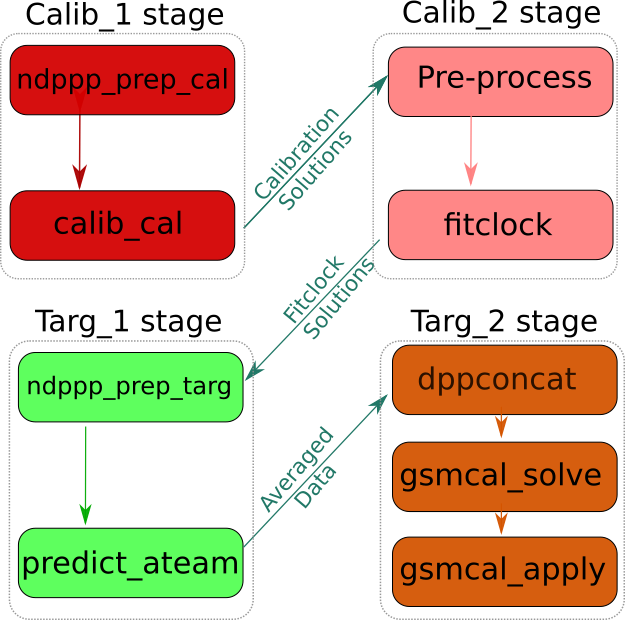
\includegraphics[width=0.95\linewidth]{figures/4_stages_steps1.png}
      \caption{The major steps of the \texttt{prefactor} DI pipeline. }
	\label{fig:prefactor_steps}
\end{figure}

\subsection{Processing Metrics}
The goal for our scalability model is to understand the effect of several parameters on the job completion time of LOFAR software. We do this by testing the processing time for various values of data size, number of CPUs used and sky model size. 

The data used by the LOFAR surveys is archived at a time resolution of 1 second intervals and frequency resolution of 16 channels per Subband (equivalent to 12kHz channel width). While some of the processing steps such as flagging of Radio Frequency Interference and removal of bright off-axis sources produce better results when performed on the high-resolution data. Later steps can be performed on averaged data with little impact on the final product quality. To speed up processing, the raw data is averaged in time and frequency, decreasing the input data size to later tasks. The main aims of the LOFAR surveys project can be accomplished if the final data products from the prefactor pipeline are averaged to a resolution of 8 seconds per sample and 2 channels per subband. These averaging parameters correspond to a reduction in size by a factor of 64. In Section \ref{sec:results_size}, we measure the performance of the \texttt{prefactor} pipeline for data sizes between the raw data of 64GB/Subband and the averaged data of 1GB/Subband. The tested data sizes and parameters are shown in table \ref{table:averaging}. 


\begin{table}[!ht]
\centering
\begin{tabular}{||c| c | c | c||} 
 \hline
 Data set & \multicolumn{1}{|p{2cm}|}{\centering Time averaging \\ parameter (sec)} &  \multicolumn{1}{|p{2cm}|}{\centering Channels per Subband} & Size (Gb) \\ [0.5ex]
 \hline
 \rowcolor{Gray}
  \hline
 1GB & 8   & 2   &  1.235   \\ 
  \hline
 2GB & 4   & 2   &  2.459   \\ 
 4GB & 2   & 2   &  4.906   \\ 
 8GB & 1   & 2   &  9.802   \\ 
 16GB & 1   & 4   &  18.00  \\ 
 32GB & 1   & 8   &  36.72  \\ 
 64GB & 1   & 16   &  66.88  \\[1ex] 
 \hline
\end{tabular}
\caption{Averaging parameters and final data sizes tested for the sample LOFAR SKSP observation. The raw data is 64 GB per Subband. The LOFAR SKSP data processing uses averaging parameters of 8 seconds and 2 channels per Subband. This reduces the raw data by a factor of 64. We highlight the data size used in the LOFAR SKSP survey.   }
\label{table:averaging}
\end{table}

The slowest step of the \texttt{prefactor} pipeline is the gsmcal\_solve step, which performs the gain calibration against a model of the radio sky. This step operates on a concatenated data set that consists of 10 subbands. We obtain the calibration model through the TGSS sky model creator\footnote{Accessible at \href{http://tgssadr.strw.leidenuniv.nl/doku.php}{the TGSS ADR portal}.}. By default this service creates a text file describing the sky-model from the TGSS survey \citep{tgssadr}. By default, it sets a threshold of sources brighter than 0.3 Jy. 
Lowering this threshold creates longer sky-model files with more faint sources, while increasing it will return only the few brightest sources. Since sky model calibration requires converting the sky-model into modelled visibilities \citep[e.g.][]{dppp, radio_visibility_sage,app_synth}, a longer sky model will increase the time taken to gain calibrate a data set. We created 7 sky models with a flux cutoff ranging between 0.05 Jy and 1.5 Jy. The number of sources in the resulting models are listed in Table \ref{table:skymodels}. 
For production\footnote{The query used to obtain model 3 is at the following link \url{http://bit.ly/tgss_model}}, we used the minimum sensitivity parameters for model 3.
%%%%%Each line of these model files corresponds to one source, modelled either as a point or an ellipse), hence the second column also lists the number of sources per sky model file. %Suggested remove by Huub

It is important to note that the complexity and accuracy of the sky model depend on the direction of observation and the conditions in which the observation was performed. As such, our test is only a heuristic for predicting the run-time based on the calibration model length. Additionally, it is notable that the number of sources is an exponentially dependent on the minimum sky model sensitivity (seen in Figure \ref{fig:skymodel_size}, more in \citealt{tgssadr,Wendy_bootes}). According to this relationship, even a modest decrease in sensitivity cutoff can significantly decrease the size of the model.

\begin{table}[!ht]
\centering
\begin{tabular}{||c| c | c||} 
 \hline
 Sky model \# & min sensitivity & \# sources  \\ [0.5ex] 
 \hline
 model 1 & 0.05 Jy & 809    \\ 
 model 2 & 0.1 Jy & 503   \\
 \rowcolor{Gray}
  \hline
 model 3 & 0.3 Jy & 180   \\
  \hline
 model 4 & 0.5 Jy & 96  \\
 model 5 & 0.8 Jy & 49   \\ 
 model 6 & 1.0 Jy & 34   \\
 model 7 & 1.5 Jy & 16   \\[1ex] 
 \hline
\end{tabular}
\caption{List of test sky models. Model 3 is created with the parameters used in our production processing of LOFAR data. All models include objects within 5 degrees from the centre of the pointing.  }
\label{table:skymodels}
\end{table}


\begin{figure}
    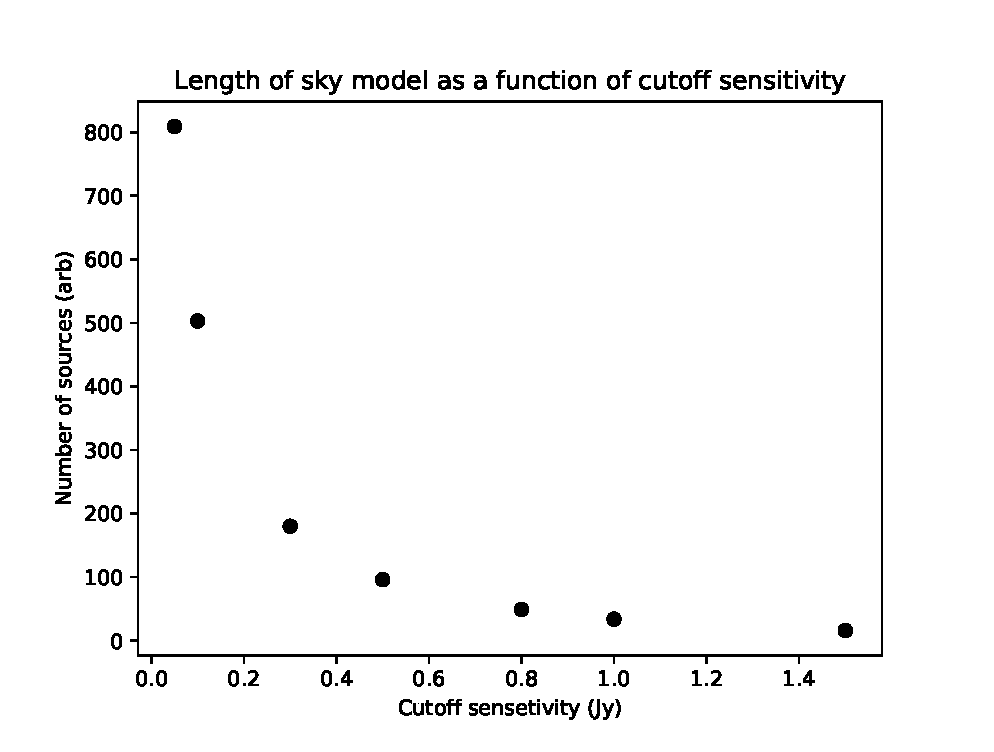
\includegraphics[width=0.95\linewidth]{figures/skymodel_size_vs_Jy.eps}
      \caption{The size of the sky model (measured in number of sources) increases exponentially as we decrease the flux cutoff of the model (i.e. increase the sensitivity).}
	\label{fig:skymodel_size}
\end{figure}


Finally, the number of CPUs used by each step is a parameter that can be optimized for the entire pipeline. While increasing the number of CPUs can make some steps run faster, requesting jobs that reserve a large number of CPUs will take longer to launch on shared infrastructure. In order to understand the interplay between these effects, we study the queuing time and processing time as a function of number of CPUs. For the parameter steps we choose to test 1, 2, 3, 4, 8 and 16 CPUs. 

\subsection{Infrastructure Performance}
%%%%%Staging files at different locations can be modelled using historical data, discuss the importance of knowing the time it takes to stage data and the prediction of future performance. 

Since our jobs are launched on a cluster supporting several different use cases, the requested resources are allocated by a job queue, in our case implemented by the glite workload management system \citep{glite-wms}. As queuing jobs can take a significant amount of time, we test the queuing time as a function of number of requested CPUs. In order to do that, we create test jobs that log the launch time and submit them, requesting 1, 2, 3, 4, 8 and 16 CPUs. We run 10 to 15 tests for each parameter step to ensure that we capture system variability at different times of day during the week and the weekend. 

Besides queuing, time is also spent during downloading and unpacking data, as well as packing and uploading the results. Despite using no compression to pack the data, untarring and tarring large files still takes time depending on the system workload. We measure the time taken to transfer and unpack data of different sizes. The data sizes we chose were 0.5GB, 1GB, 2GB, 4GB, 8GB, 16GB, 32GB and 64GB. As our largest data sets are 64GB and our smallest results are $\sim$0.2GB, these values span a realistic range expected for LOFAR data processing. We test this by uploading mock data to the dCache storage pool at SURFsara and launching a small 1 CPU job which downloads and untars the data, logging the start time of each step. We present the results of this test in the next section. 


\subsubsection{Software Versions}\label{sec:software_versions}
For the current test, we use the LOFAR software stack, version 2.20.2 \citep{cookbook}. This software was compiled on a virtual machine and distributed using the CERN CVMFS virtually mounted file system \citep{cvmfs2008}. We use this software version and distribution method as it is the same software version and distribution used to process the data for the LOTSS Data Release 1. 

\subsection{Test Hardware}\label{sec:hardware}

The LOFAR software was tested on a reserved node on the SURFsara \texttt{GINA} cluster. The node, f18-01 has 348 GB of RAM, 3TB of scratch space\footnote{More detailed specifications are at \href{http://docs.surfsaralabs.nl/projects/grid/en/latest/Pages/Service/system_specifications/gina_specs.html}{the \texttt{GINA} specification page linked here}}. The CPU is an Intel Xeon(R) Gold 6148 CPU with 40 cores clocked at 2.40GHz.  As this hardware node was reserved, there was no other scientific processing aside from our tests, meaning there was no resource contention aside for that inherent in the LOFAR software. In the results section, we compare these isolated runs with processing results over the past two years. 

\section{Results}\label{sec:results}

Using a test data set, we tested the LOFAR \texttt{prefactor} target pipeline on the SURFsara \texttt{GINA} cluster. First we'll present the tests done in an isolated environment and then compare them to the run time in production on a shared infrastructure. Finally, we'll make some predictions on the run time of our processing based on the model and validate these predictions. 

Since we're processing a sample data set in the context of the LOFAR Surveys project, these tests can be compared with the production runs of our pipeline. In production, the parameters chosen are a data size of 1.3GB, a sky model length of 180 lines and 8 CPUs for the gsmcal\_solve step. 


\subsection{Isolated Environment tests}
We first tested the LOFAR software in isolation in order to determine the scalability of processing time in terms of data size. The slowest step for \texttt{prefactor} processing is the gsmcal\_solve step. This task performs gain calibration of the averaged data against a sky model, determining the gain parameters that minimize the difference between the data and the model. As an input, this step takes the averaged data and a model of the radio sky as a text file. 

\subsubsection{Input Data Size}\label{sec:results_size}
LOFAR data can be averaged to different sizes based on the scientific requirements. Smaller data sets are processed faster, so it is important to understand the effect of data size on processing time. Figures \ref{fig:dpppconcat_size}, \ref{fig:gsmcalsolve_size} and \ref{fig:gsmcalapply_size}  show the processing time for our test data set, averaged to different sizes for the slowest \texttt{prefactor} steps. Figures \ref{fig:predict_ateam}, \ref{fig:ateamcliptar}, \ref{fig:dpppconcat_size}, \ref{fig:gsmcalsolve_size}, \ref{fig:gsmcalapply_size} show the scaling relation between the run time and data size for these steps. 

With minor deviations, all of the steps show linear behavior with respect to input data size. The linear fit to the run times are shown in Equations \ref{eq:predictateam}-\ref{eq:gsmcalapply}. The equations show the processing time as a function of the data size, with the slope in the units of seconds/byte.

\begin{subequations}
\begin{align}
        y_{predict\_ateam}=5.19\cdot10^{-8}x+4.20\cdot10^1 \label{eq:predictateam} \\
        y_{ateamcliptar}=4.57\cdot10^{-9}x-8.42\cdot10^0 \label{eq:ateamcliptar} \\
        y_{dpppconcat}=3.51\cdot10^{-8}x+4.20\cdot10^1 \label{eq:dpppconcat} \\
        y_{gsmcal\_solve}=9.97\cdot10^{-7}x-1.56\cdot10^3 \label{eq:gsmcalsolve} \\
        y_{gsmcal\_apply}=2.07\cdot10^{-8}x-1.38\cdot10^1 \label{eq:gsmcalapply}
\end{align}
\label{eq:runtime_size_models}
\end{subequations}

%predict\_ateam::  R=9.958E-01 and stderr=1.919E-10
%ateamcliptar ::  R=9.786E-01 and stderr=3.945E-11
%dpppconcat :: R=9.988E-01 and stderr=1.757E-10
%gsmcal\_solve ::   R=9.969E-01 and stderr=7.983E-09
%gsmcal\_apply ::   R=9.893E-01 and stderr=3.121E-10

\begin{figure}
    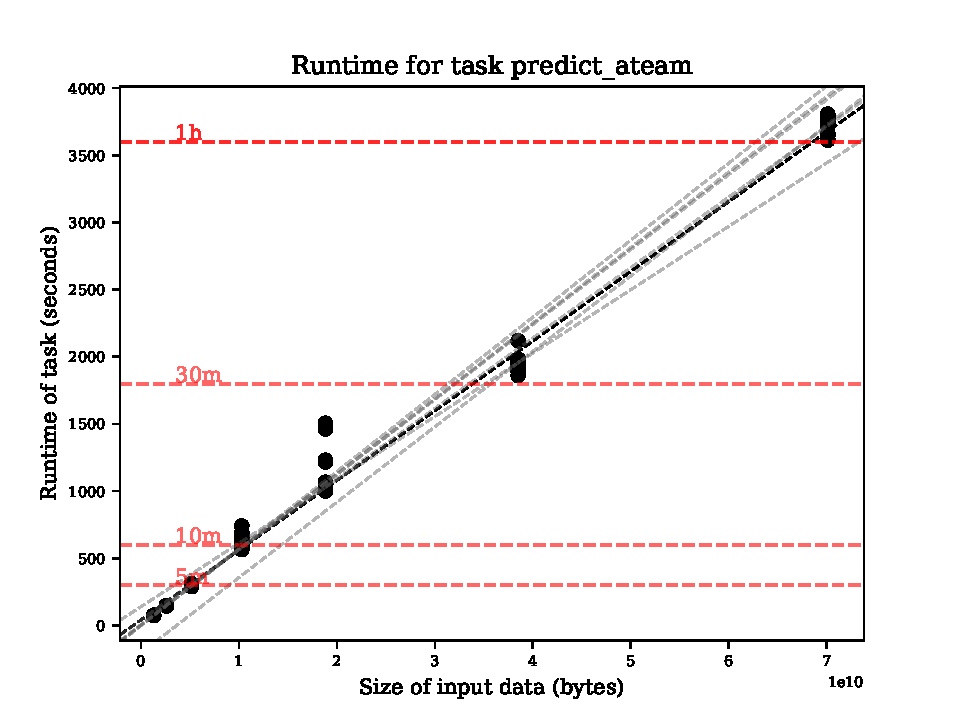
\includegraphics[width=0.95\linewidth]{figures/predict_ateam_size.pdf}
      \caption{Tests of the predict\_ateam step for input data size ranging from 1GB to 64 GB. This step calculates the contamination from bright off-axis sources. Dashed lines are shown connecting each pair of points, to highlight the trend. The linear model fit to this data (Equation \ref{eq:predictateam}) is shown in black. }
	\label{fig:predict_ateam}
\end{figure}


\begin{figure}
    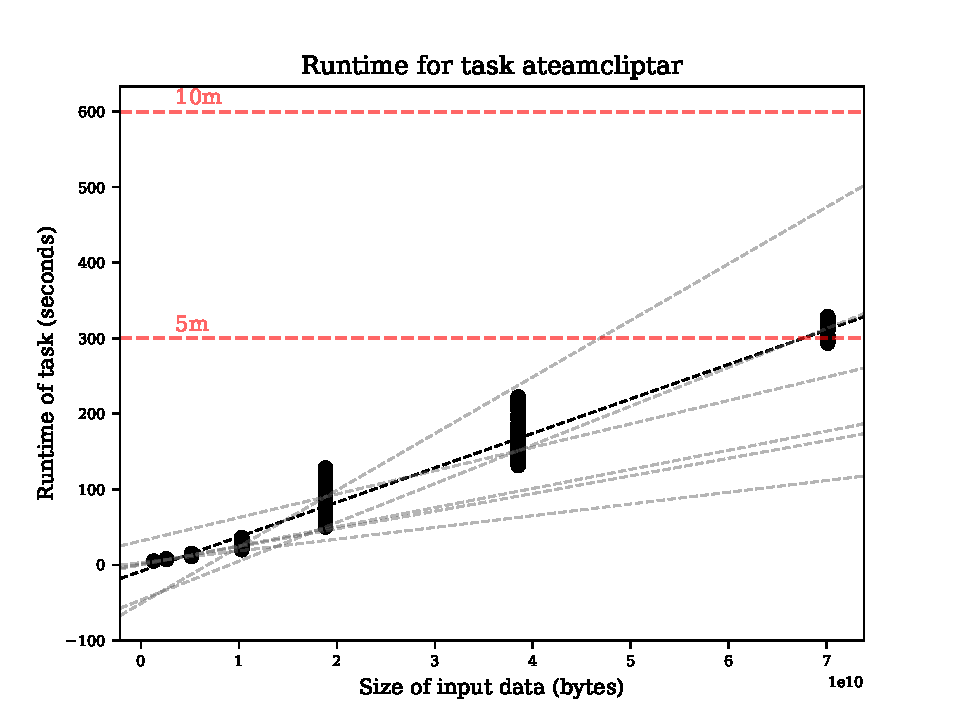
\includegraphics[width=0.95\linewidth]{figures/ateamcliptar_size.pdf}
      \caption{Tests of the ateamcliptar step for input data size ranging from 1GB to 64 GB. This step removes the contamination from bright off-axis sources. The linear model fit to this data (Equation \ref{eq:ateamcliptar}) is shown in black.}
	\label{fig:ateamcliptar}
\end{figure}

\begin{figure}
    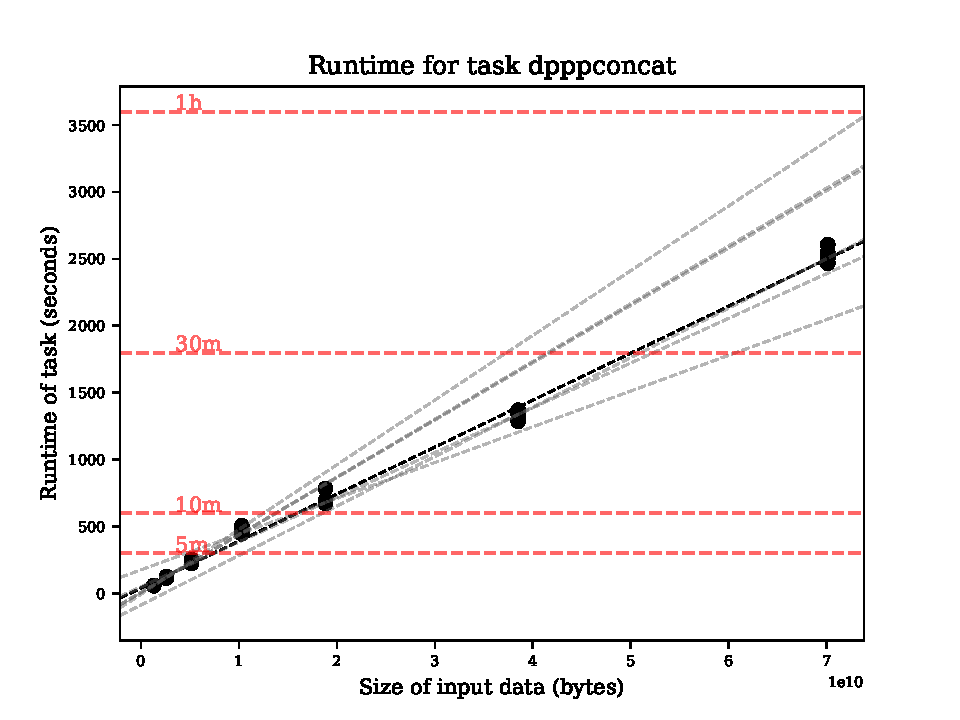
\includegraphics[width=0.95\linewidth]{figures/dpppconcat_size.pdf}
      \caption{Tests of the dpppconcat step for input data size ranging from 1GB to 64 GB. This step concatenates 10 files into a single measurement set. The linear model fit to this data (Equation \ref{eq:dpppconcat}) is shown in black.}
	\label{fig:dpppconcat_size}
\end{figure}


\begin{figure}
    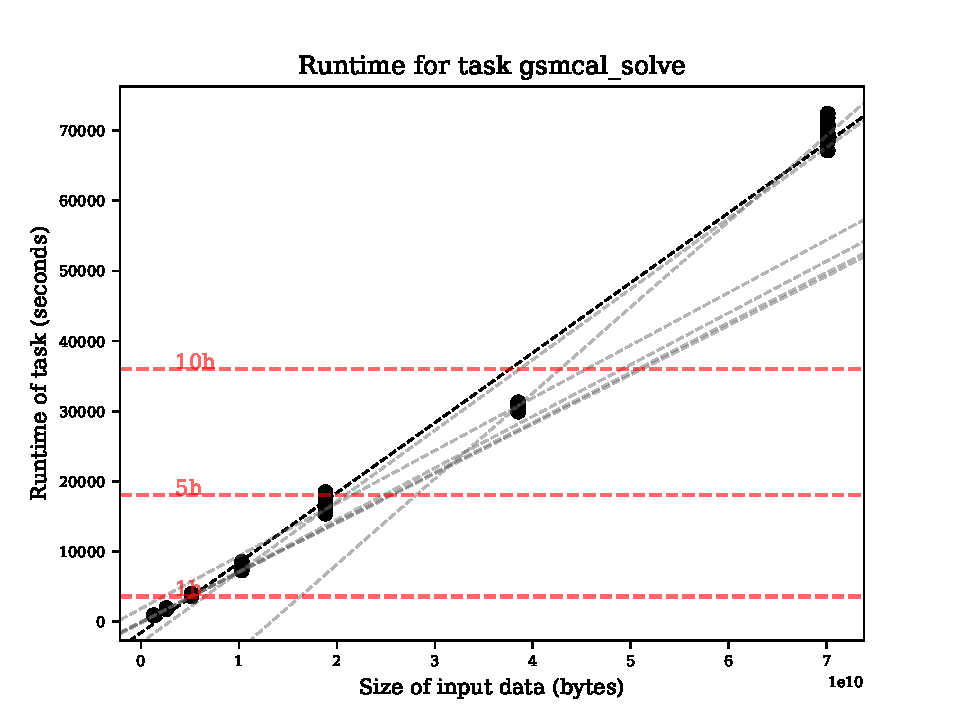
\includegraphics[width=0.95\linewidth]{figures/gsmcal_solve_size.pdf}
      \caption{Tests of the gsmcal\_solve step for input data size ranging from 1GB to 64 GB. This step performs gain calibration of the concatenated data set against a sky model. It is the slowest and most computationally expensive \texttt{prefactor} step. The linear model fit to this data (Equation \ref{eq:gsmcalsolve}) is shown in black.  }
	\label{fig:gsmcalsolve_size}
\end{figure}

\begin{figure}
    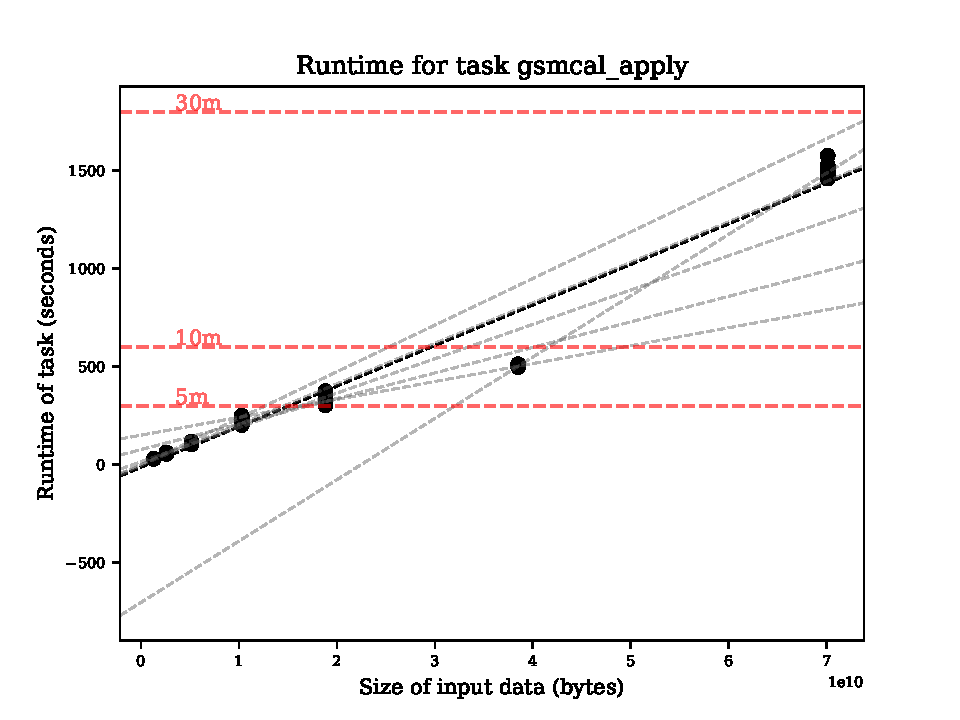
\includegraphics[width=0.95\linewidth]{figures/gsmcal_apply_size.pdf}
      \caption{Tests of the gsmcal\_apply step for input data size ranging from 1GB to 64 GB. This step applies the calibration solutions to the data. The linear model fit to this data (Equation \ref{eq:gsmcalapply} is shown in dark blue.}
	\label{fig:gsmcalapply_size}
\end{figure}

\subsubsection{Global Sky Model Size}
To test the effect of the calibration model size on run time, we tested our calibration with several different lengths of the sky model file. We tested sky models ranging in sensitivity from 0.05 Jy to 1.5 Jy. The most sensitive model had 809 sources while the 1.5 Jy model had only 16 sources. 

Figure \ref{fig:skymodel_run_lenght} shows that the calibration time is directly proportional to the length of the sky model. Figure \ref{fig:skymodel_run_sens} shows the run time as a function of the processing parameter: the cutoff sensitivity. As the relationship between the number of sources and sensitivity is a power law, here we see the same relationship holding for processing time.

We model the run time as a function of the cutoff frequency using a power law, and fit the data to the function $y=\alpha\cdot x^{-k}$. Our fit found the best model to be shown in Equation \ref{eq:skymodel_flux}, where $x$ value is the cutoff flux in Jansky and $y$ is the run time in seconds. 

\begin{equation}
    y=1185\cdot x^{-0.854}
\label{eq:skymodel_flux}
\end{equation}

\begin{figure}
    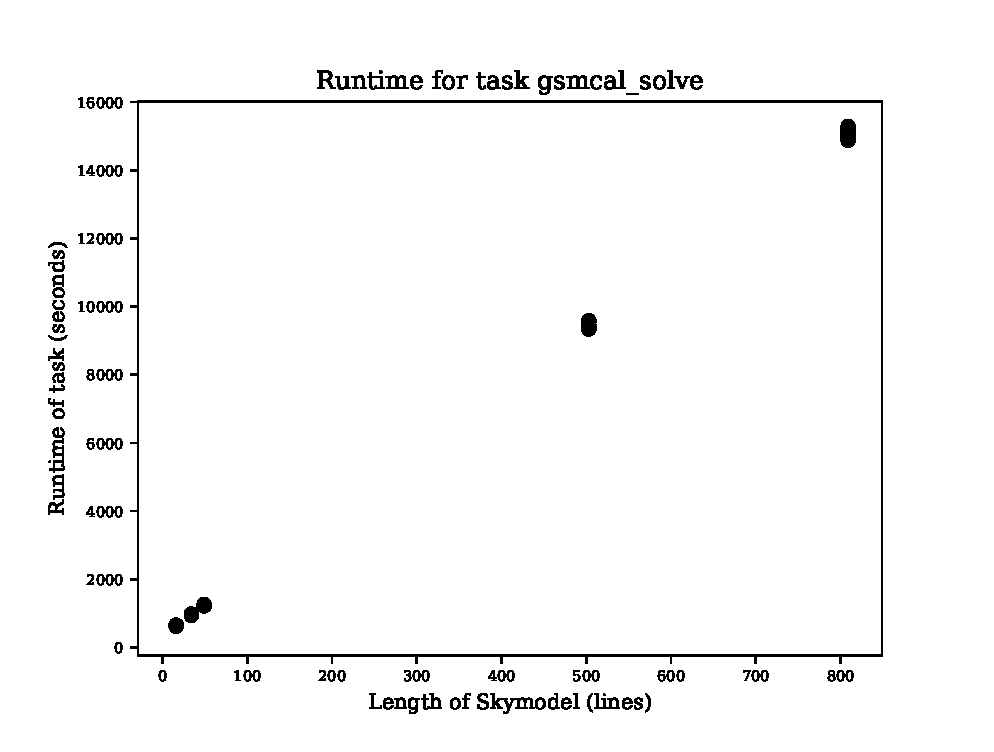
\includegraphics[width=0.95\linewidth]{figures/skymodel_length.eps}
      \caption{The processing time of the gsmcal\_solve step is linear with the size of the sky model as measured by the number of sources.}
	\label{fig:skymodel_run_lenght}
\end{figure}

\begin{figure}
    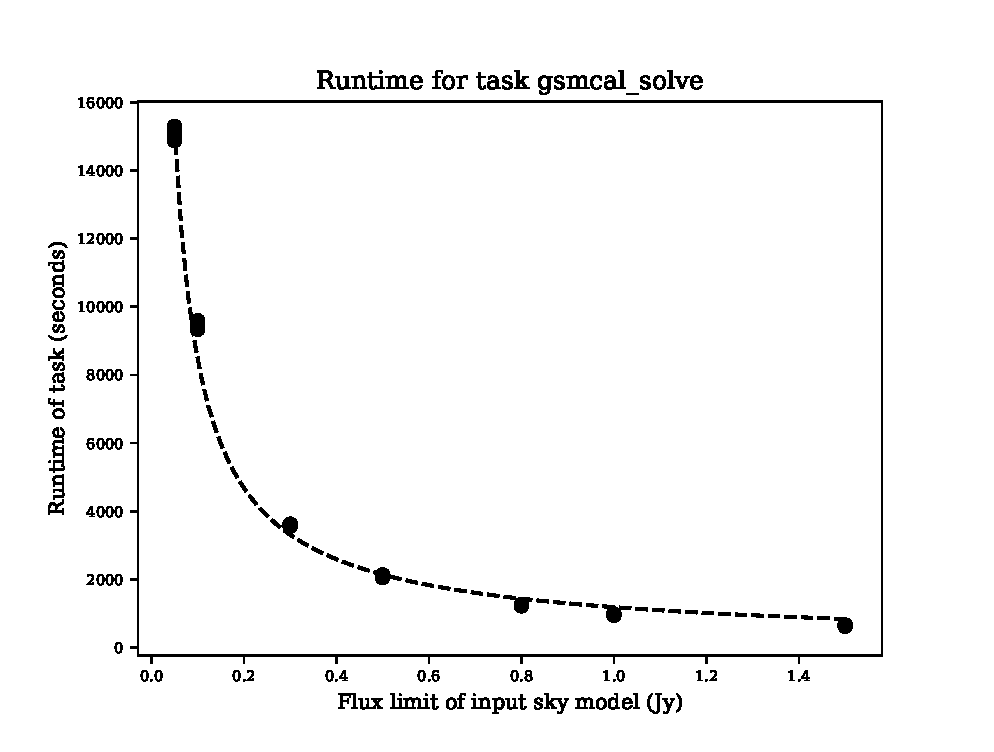
\includegraphics[width=0.95\linewidth]{figures/skymodel_flux.eps}
      \caption{The run time of the gsmcal\_solve step as a function of the cutoff sensitivity is not linear. As shown in Figure \ref{fig:skymodel_size}, the number of sources increases exponentially as the minimum sensitivity decreases. The dashed line shows the model fitted in equation \ref{eq:skymodel_flux}. }
	\label{fig:skymodel_run_sens}
\end{figure}

\subsubsection{Number of CPUs}
One parameter that can be optimized is the number of CPUs requested when the job is launched. We investigated the processing speedup as a function of the number of CPUs for the \texttt{prefactor} target pipeline. 


\subsubsection{Comparison with production runs}
Over the past two years, the LOFAR software has been running in production and collecting data on run time for each processing step. We can compare this to the isolated model in order to determine the overhead incurred by processing LOFAR data on shared nodes. 

\subsection{Queuing Tests}

Aside from performance of the LOFAR software, we measured the queuing time at the \texttt{GINA} cluster, as a function of the number of CPUs requested. This data was obtained between 16 Nov 2018 and 10 Dec 2018 for 1, 2, 3 ,4, 8, and 16 CPUs per job. A histogram of the queuing time for these jobs is shown in Figure \ref{fig:queue_NCPU}.

\begin{figure}
    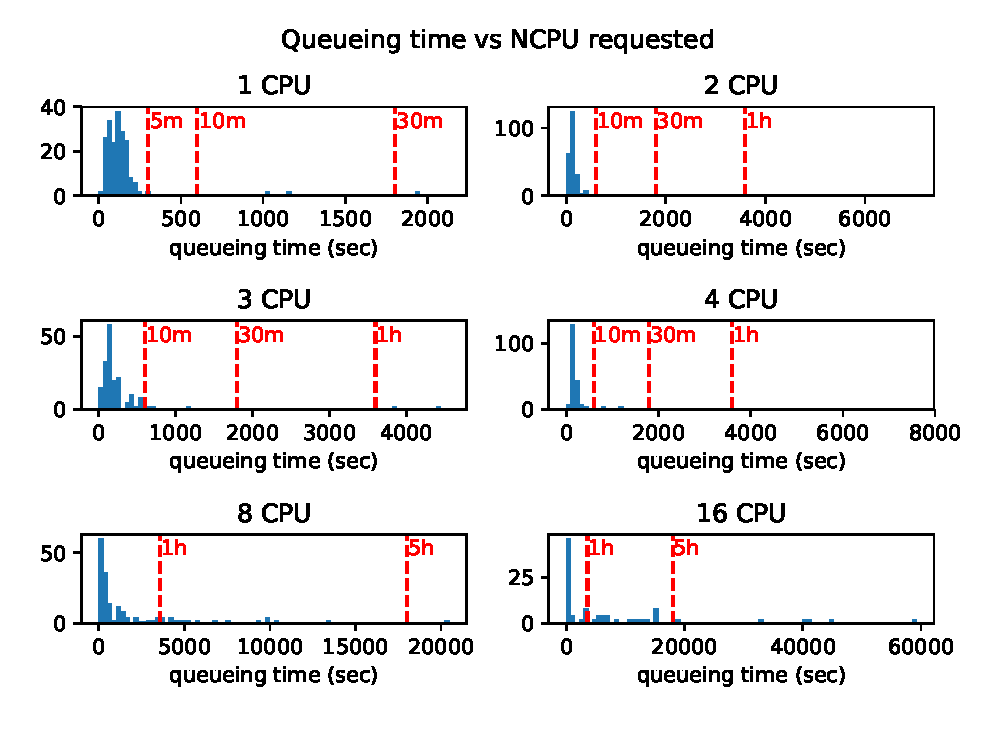
\includegraphics[width=0.95\linewidth]{figures/Queue_NCPU.eps}
      \caption{Test randomly submitting jobs to the \texttt{GINA} with different number of requested CPUs. Outliers due to grid downtime have been removed \textbf{Actually do this though} }
	\label{fig:queue_NCPU}
\end{figure}


\subsection{Transfer and Unpacking Time}

We tested the downloading and unpacking time for data sizes ranging from 512MB to 64GB. We discovered that the unpacking of files below 64GB scaled linearly with file size, however unpacking data larger than 16GB becomes considerably slower than downloading it. 

Figure \ref{fig:dl_hist} shows the histogram of the download tests, and Fig \ref{fig:dl_plot} displays the tests as a function of data size. Both figures show that extracting of the 32 and 64GB data sets has more slow outliers than the downloading of this data. 

\begin{figure}
    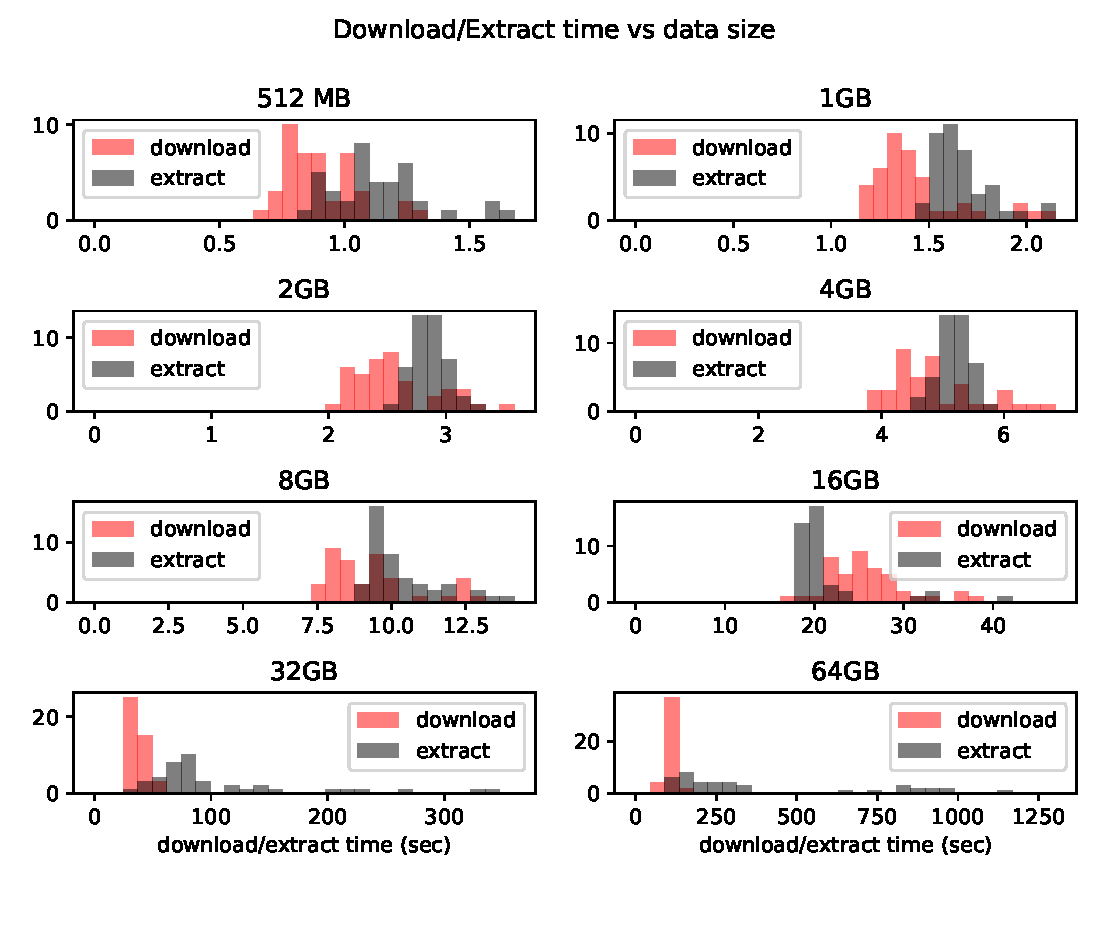
\includegraphics[width=0.95\linewidth]{figures/dl_ex.pdf}
      \caption{A histogram of the download and extracting times of multiple data sizes on the \texttt{GINA} worker nodes. Download and extract times are comparable for data up to 8GB, however above that, the extracting time dominates.  }
	\label{fig:dl_hist}
\end{figure}

\begin{figure}
    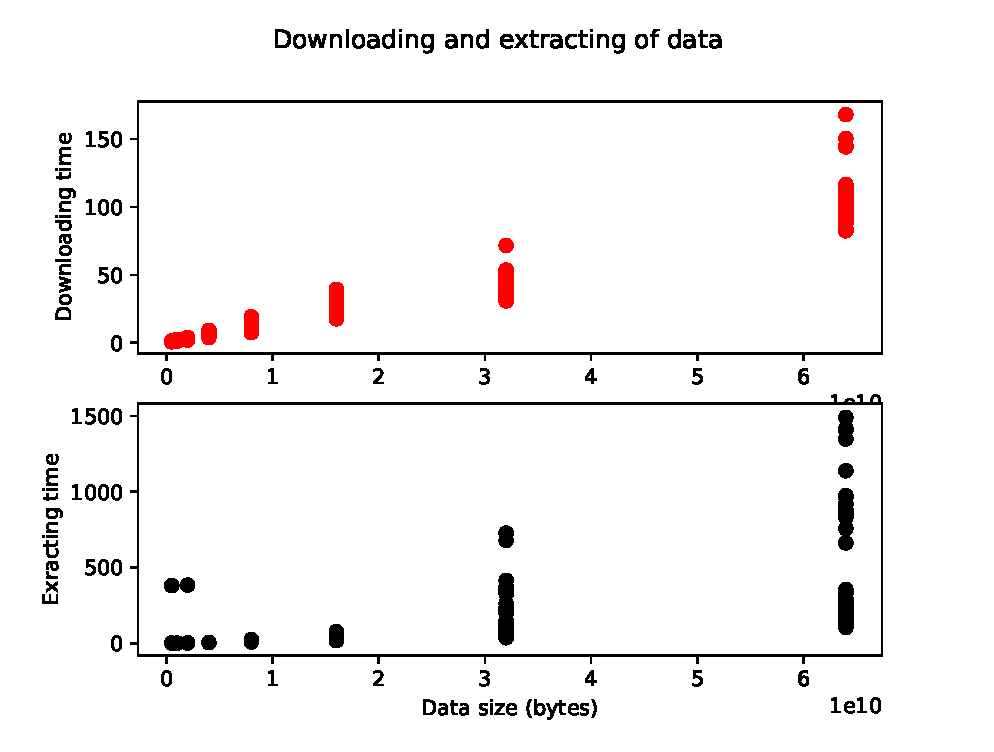
\includegraphics[width=0.95\linewidth]{figures/download_extract_sct.eps}
      \caption{A scatter plot of the download and extracting times of multiple data sizes on the \texttt{GINA} worker nodes. The difference between download and extract time for the 32 and 64 GB data sets can be seen.  }
	\label{fig:dl_plot}
\end{figure}


\subsection{Validation}
Test some data sets outside of the model and see if it can predict performance. 


\section{Discussions and Conclusions}

We scaled the size of broadband LOFAR data by a factor of 64 in size, and discovered that all our processing steps scale linearly in time with respect of the input data size. The largest data set tested, a measurement set of 64 GB, appears to lie above this trend. This may be because of resource contention for this test case. \textbf{(Will investigate)}

Overall, the slowest step was the gsmcal\_solve step, and its run time scales more strongly with data size than the other steps (equation \ref{eq:gsmcalsolve} has the steepest slope). This suggests that as data sizes increase, gsmcal\_solve will increasingly dominate the processing time over the other steps (As seen in Figures \ref{fig:gsmcalsolve_size} and \ref{fig:predict_ateam}.)

Additionally, we tested the calibration time as a function of input sky model length and sensitivity. It was discovered that the calibration scales linearly in time as a function of number of lines, however it is a power law as a function of the cutoff sensitivity. This is because of the (expected) power law relation between the number of sources and cutoff sensitivity, seen in Figure \ref{fig:skymodel_size}. This discovery can be used to accelerate the processing time by increasing the flux cutoff to the LOFAR direction independent calibration to 0.5 Jy. Doing so will execute the calibration step in 60\% of the time, saving 83 CPU-h per run. Over the remaining 2000 \texttt{prefactor} runs left in the LOTSS project, this change in sensitivity will save more than 167k CPU hours. \textbf{Show images and calibration solutions to convince it's "OK"}

We tested downloading and extracting test LOFAR data of various sizes. Both downloading and extracting was linear with respect to the data size for data up to 32 GB in size. Beyond that scale, extracting data could take much slower than the trend. This is because load on the worker node's file-system can be variable.


Part of the LOFAR SKSP processing is done on shared infrastructure, which requires requesting processing time ahead of time for each grant period. Being able to predict the amount of resources required to process data each grant period is required to make a reliable estimate on what resources to request.

Moreover, to provide LOFAR processing as a service to scientific users, it is important to estimate the processing time for each request. This needs to be done in order to determine whether the user has sufficient resources left in their resource pool. Knowing the performance of the software pipelines as a function of the input parameters will help predict the run time for each request and the resources consumed. Knowing this will make it possible to notify users how long the request will take and warn them of how much of their quota will be used up. 

Finally, a performance model of the LOFAR software will help make predictions on the time and resources needed to process data for other telescopes such as the Square Kilometer Array (SKA). Once operational, the SKA is expected to produce Exabytes of data per year. Processing this data efficiently requires understanding the scalability of the software performance to facilitate scheduling and resource allotment. Overall, these results will help guide algorithm development in radio astronomy, as well as be useful to schedule future processing jobs and optimize resource usage. 


\appendix

\renewcommand{\theequ}{\Alph{section}.\arabic{equ}}


\section{Calibration Solutions for the sky model tests }\label{ap:calib_solutions}
The output of the calibration step is a data set corrected for direction independent effects, as well as a set of calibration solutions. Figures \ref{fig:skymodel_rcalib_004_03} and \ref{fig:skymodel_rcalib_08_15} show the calibration solutions for core stations obtained when calibrating with sky models with minimum flux cutoffs of 0.05, 0.3, 0.8 and 1.5Jy. Much like in Figure \ref{fig:skymodel_images}, we can see that there is no significant difference between the calibration solutions for these stations. As a note, the naming scheme for LOFAR stations is CS/RS for core/remote stations, three digits for station number, HBA0/HBA1 for High Band antennas and LBA0/LBA1 for low-band antennas. The 0,1 suffixes correspond to sub-arrays in the core stations which can be correlated separately. Additionally, the CS/RS is replaced with the 2-letter country code for international stations\citep{staiton_data_cookbook}.

We compare the phase solutions for stations CS032HBA0 and CS003HBA0 and the reference station for two different calibrations in Figure \ref{fig:diffs_solutions}. We note that this difference is within 0.3 rad for the entire observation. Combined with the results in the other two plots, our results suggest that the calibration solutions do not degrade when calibration is done with a smaller sky model.

\begin{figure}
    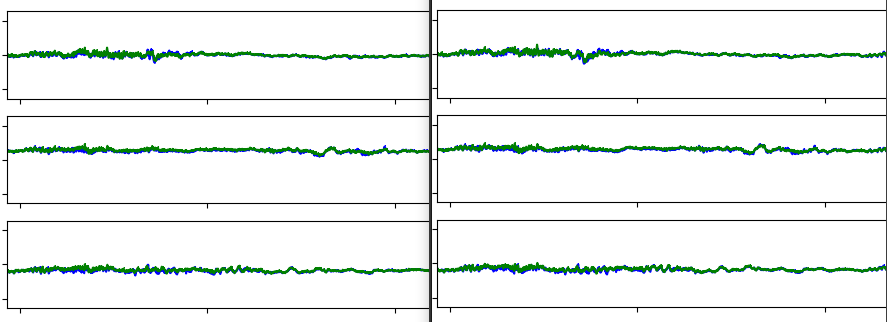
\includegraphics[width=0.95\linewidth]{figures/005_and_03_solutsions_CS003HBA0_CS003HBA1_CS004HBA0.png}
      \caption{The calibration (phase) solutions for the test dataset obtained when calibrating with sky models of 0.05 Jy cutoff (left) and 0.3Jy cutoff (right). The data shows the phase solutions for baselines including stations CS003HBA0, CS003HBA1 and CS004HBA0, with respect to the reference station, CS001HBA0. The right solutions were obtained using the production calibration model. We do not see any improvement in results in the left figure, which took twice as long to obtain.}
	\label{fig:skymodel_rcalib_004_03}
\end{figure}

\begin{figure}
    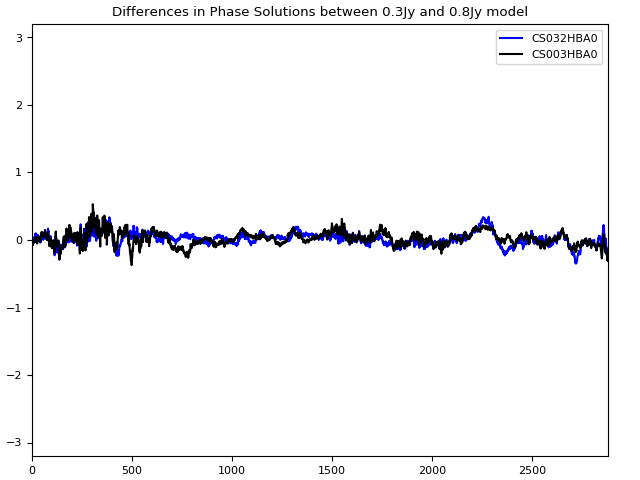
\includegraphics[width=0.9\linewidth]{figures/diffs.png}
      \caption{Difference of phase solutions between calibrations with the 0.3Jy and 0.8Jy sky models. The solutions for both stations are around zero phase for the duration of the observation.}
	\label{fig:diffs_solutions}
\end{figure}

\begin{figure}
    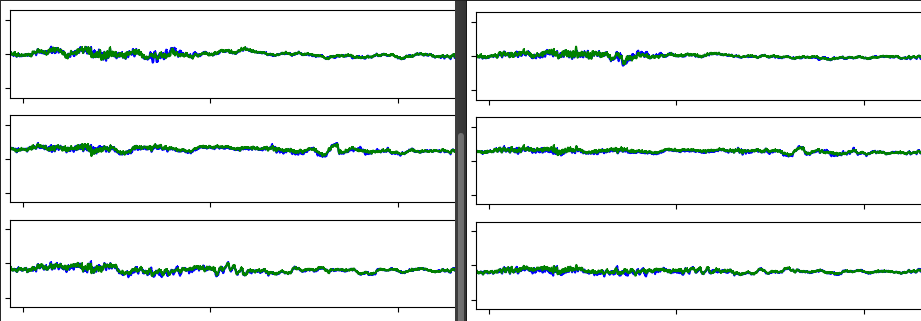
\includegraphics[width=0.95\linewidth]{figures/08_and_15_solutsions_CS003HBA0_CS003HBA1_CS004HBA0.png}
      \caption{The calibration (phase) solutions for the test dataset obtained when calibrating with sky models of 0.8 Jy cutoff (left) and 1.5Jy cutoff (right). The data shows the phase solutions for baselines including stations CS003HBA0, CS003HBA1 and CS004HBA0, with respect to the reference station, CS001HBA0. We can see that the calibration solutions shown here are not significantly different than those shown in \ref{fig:skymodel_rcalib_004_03}, despite taking a fraction of the processing time.  }
	\label{fig:skymodel_rcalib_08_15}
\end{figure}

\section{Parametric model parameters and fit accuracy}\label{ap:model_params}

In this section, we note the uncertainties to the models fit in Equations \ref{eq:runtime_size_models}-\ref{eq:download_model}. 

%Resetting the equation environment to match the equ number
\numberwithin{equation}{section}
\setcounter{equation}{6}
\renewcommand{\theequation}{\Alph{section}.\arabic{equation}}

\subsection{Fits quality of run time vs input size model}

The models of the processing time vs input size were fit as a linear regression. In this work we present such models for the {\fontfamily{qcr}\selectfont  gsmcal\_solve}, {\fontfamily{qcr}\selectfont gsmcal\_apply}, {\fontfamily{qcr}\selectfont dpppconcat}, {\fontfamily{qcr}\selectfont predict\_ateam} and {\fontfamily{qcr}\selectfont ateamcliptar}, the five slowest steps. The resulting models, calculated by the \texttt{scipy linregress}\citep{scipy} routine, are shown in Equation \ref{eq:runtime_size_models}. We present the $R^2$ values, P values and standard error below, in Table \ref{table:fits_size}.



\begin{table}[ht!]
\centering
\begin{tabular}{||p{2.2cm}| c | c|p{2cm}||} 
 \hline
 \texttt{prefactor} step & $R^2$ & P value & Standard Error \\ %[0.5ex]
 \hline
 predict\_ateam & 0.996   & 0                    & $1.92\times10^{-10}$    \\ 
 \hline
 ateamcliptar   & 0.979   & 0                    & $3.94\times10^{-11}$    \\ 
 \hline
 dpppconcat     & 0.999   & $1.2\times10^{-128}$ & $1.78\times10^{-10}$    \\ 
 \hline
 gsmcal\_solve $<=$16GB  & 0.995   & $3.12\times10^{-75}$ & $6.80\times10^{-9}$     \\ 
 \hline
 gsmcal\_solve $>$16GB  & 0.951   & $7.07\times10^{-40}$ & $1.58\times10^{-8}$     \\ 
 \hline
 gsmcal\_apply  & 0.989   & $5.6\times10^{-82}$  & $3.12\times10^{-10}$    \\ 

\hline
\end{tabular}
\caption{Fit parameters for the models in Equation \ref{eq:runtime_size_models}. }
\label{table:fits_size}
\end{table}


\subsection{Fit of run time vs calibration model flux cutoff }

The run time vs Flux cutoff model shown in Equation \ref{eq:skymodel_flux} is defined by the equation $y=a\cdot x^{-k}$ and two parameters, $a$ and $k$. The covariance matrix for these two parameters is shown in Equation \ref{eq:cov_Flux}. The standard deviation for the fit of the parameters $a$ and $k$ is 26.134 and $7.624\times10^{-3}$ respectively.

\begin{equ}
\begin{equation}
  \begin{bmatrix}
    6.83\times10^{2}  &  -1.94\times10^{-1} \\
   -1.94\times10^{-1} &   5.81\times10^{-5} \\
\end{bmatrix}
\end{equation}
\caption{The covariance matrix of the parameters in model in Equation \ref{eq:skymodel_flux}.}
\label{eq:cov_Flux}
\end{equ}

\subsection{Fit of the NCPU model }
The covariance matrix for the fit parameters of equation \ref{eq:gsmcal_NCPU}, $a$ and $k$ in $y=a+\frac{k}{\mathcal{N}}$ are shown in Equation \ref{eq:cov_NCPU}. The standard deviation of the fits for $a$ and $k$ are 13.11 and 48.20 respectively. 

\begin{equ}
\begin{equation}
  \begin{bmatrix}
    171.94 & -504.11 \\
    -504.11 & 2322.95
\end{bmatrix}
\end{equation}
\caption{The covariance matrix for the parameters for the model predicting run time vs Number of CPUs used, shown in Equation \ref{eq:gsmcal_NCPU}.}
\label{eq:cov_NCPU}
\end{equ}

\subsection{Fit for the queuing time model}

The statistics of the model fit parameters for the queuing time model (Equation \ref{eq:queue_model}) are in Table \ref{table:fits_queue}. 
The queuing model is fit to the $75^{th}$ percentile of the queuing times for each parameter step. Since this results in a single number for each step, the model's P values are larger than the models from the other sections. 

\begin{table}[ht!]
\centering
\begin{tabular}{||p{2.2cm}| c | c|p{2cm}||} 
 \hline
 Value of $\mathcal{N}$ & $R^2$ & P value & Standard Error \\ %[0.5ex]
 \hline
 $\mathcal{N}\leq4$ & 0.382   & 0.381                   & 37.086    \\ 
 $\mathcal{N}>4$    & 0.986   & 0.075                   & 86.293    \\ 
\hline
\end{tabular}
\caption{Goodness of fit parameters for the model in Equation \ref{eq:queue_model}. Since the model is split into two parts, we treat each section as a single linear model.}
\label{table:fits_queue}
\end{table}


\subsection{Fit of the download and extract model }
Equation \ref{eq:cov_downl} shows the covariance matrix for the two parameters  $a$ and $k$, $y=a\times10^{k}$ with the best fit values shown in Equation \ref{eq:download_model}. The standard deviations of the fits for $a$ and $k$ are 0.016 and 0.068 respectively. 

\begin{equ}
\begin{equation}
  \begin{bmatrix}
    2.53\times10^{-4} & 1.08\times10^{-3} \\
    1.08\times10^{-3} & 4.60\times10^{-3}
\end{bmatrix}
\end{equation}
\caption{The covariance matrix for the parameters for the model for Download and Extract time, shown in Equation \ref{eq:download_model}.}
\label{eq:cov_downl}
\end{equ}


\section*{Acknowledgements}
APM would like to acknowledge the support from the NWO/DOME/IBM programme ``Big Bang Big Data: Innovating ICT as a Driver For Astronomy'', project \#628.002.001.

%Author5 gratefully acknowledge support from the European Research Council under the European Unions Seventh Framework Programme (FP/2007-2013)/ERC Advanced Grant NEWCLUSTERS- 321271.

%Author3 acknowledges financial support from NWO Top LOFAR-CRRL project, project No. 614.001.351. R.J.W. is supported by a Clay Fellowship awarded by the Harvard-Smithsonian Center for Astrophysics. AGGMT acknowledges support through the Spinoza premie of the Dutch Science Organization (NWO).

This work was carried out on the Dutch national e-infrastructure with the support of SURF
Cooperative through grant e-infra 160022 \& 160152.

\section*{References}
\bibliography{bibliography}

\end{document}

%%
%% End of file `elsarticle-template-1-num.tex'.